\fancyhead[LE,RO]{\thepage}
\fancyhead[LO]{\textbf{\textsf{CHƯƠNG 1}}\quad Các hàm số và Mô hình}
\fancyhead[RE]{\textbf{\textsf{MỤC 1.1}}\quad Bốn cách biểu diễn một hàm số}

\noindent
\begin{minipage}[t]{0.26\textwidth}
    \vspace{0pt}
    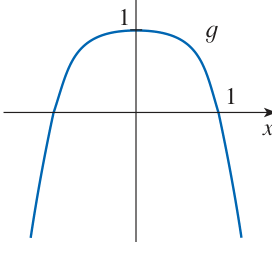
\includegraphics[width=\linewidth]{images/p0051_fig1.png}
    \vspace{-4pt}
    \captionof{figure}{\raggedright \textbf{\textsf{HÌNH 19}}\newline Một hàm số chẵn}
    \label{fig:p16_fig19}

    \vspace{1.48cm}
    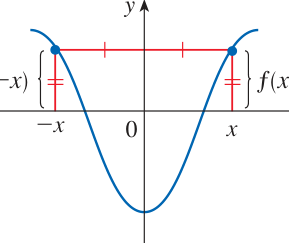
\includegraphics[width=\linewidth]{images/p0051_fig2.png}
    \vspace{-4pt}
    \captionof{figure}{\raggedright \textbf{\textsf{HÌNH 20}}\newline Một hàm số lẻ}
    \label{fig:p16_fig20}

    \vspace{5.08cm}
    \textbf{\textsf{HÌNH 21}}
\end{minipage}%
\hfill
\begin{minipage}[t]{0.71\textwidth}
    \vspace{0pt}
    Nhìn vào Hình 18, bạn có thể thấy tại sao một hàm số như trong Ví dụ 10 lại được gọi là một \textbf{hàm bậc thang} (\textit{step function}).

    \vspace{0.33cm}
    \noindent{\color{stewartcyan}\rule{6pt}{6pt}}\hspace{6pt}\textbf{\large\textsf{Hàm số chẵn và hàm số lẻ}}
    \vspace{0.16cm}

    \noindent Nếu một hàm số $f$ thỏa mãn $f(-x) = f(x)$ với mọi số $x$ thuộc tập xác định của nó, thì $f$ được gọi là một \textbf{hàm số chẵn}. Chẳng hạn, hàm số $f(x) = x^2$ là hàm chẵn vì
    \[
    f(-x) = (-x)^2 = x^2 = f(x)
    \]
    Ý nghĩa hình học của một hàm số chẵn là đồ thị của nó đối xứng qua trục $y$ (xem Hình 19). Điều này có nghĩa là nếu chúng ta đã vẽ đồ thị của $f$ với $x \geqslant 0$, ta sẽ thu được toàn bộ đồ thị chỉ đơn giản bằng cách lấy đối xứng phần đồ thị này qua trục $y$.

    Nếu $f$ thỏa mãn $f(-x) = -f(x)$ với mọi số $x$ thuộc tập xác định của nó, thì $f$ được gọi là một \textbf{hàm số lẻ}. Chẳng hạn, hàm số $f(x) = x^3$ là hàm lẻ vì
    \[
    f(-x) = (-x)^3 = -x^3 = -f(x)
    \]
    Đồ thị của một hàm số lẻ đối xứng qua gốc tọa độ (xem Hình 20). Nếu chúng ta đã có đồ thị của $f$ với $x \geqslant 0$, ta có thể thu được toàn bộ đồ thị bằng cách quay phần đồ thị này một góc $180^\circ$ quanh gốc tọa độ.

    \vspace{0.25cm}
    \noindent\textbf{\textsf{\color{stewartcyan}VÍ DỤ 11}}\quad Xác định xem mỗi hàm số sau đây là hàm chẵn, lẻ hay không chẵn cũng không lẻ.
    \begin{enumerate}[label=(\alph*), itemjoin=\qquad]
        \item $f(x) = x^5 + x$
        \item $g(x) = 1 - x^4$
        \item $h(x) = 2x - x^2$
    \end{enumerate}

    \vspace{0.16cm}
    \noindent\textbf{\textsf{\color{stewartcyan}LỜI GIẢI}}
    
    \noindent (a)
    \begin{align*}
        f(-x) &= (-x)^5 + (-x) = (-1)^5 x^5 + (-x) \\
              &= -x^5 - x = -(x^5 + x) \\
              &= -f(x)
    \end{align*}
    Do đó $f$ là một hàm số lẻ.

    \vspace{0.08cm}
    \noindent (b)
    \[
    g(-x) = 1 - (-x)^4 = 1 - x^4 = g(x)
    \]
    Vậy $g$ là hàm số chẵn.

    \vspace{0.08cm}
    \noindent (c)
    \[
    h(-x) = 2(-x) - (-x)^2 = -2x - x^2
    \]
    Vì $h(-x) \neq h(x)$ và $h(-x) \neq -h(x)$, ta kết luận rằng hàm số $h$ không chẵn cũng không lẻ. \hfill{\color{stewartcyan}$\blacksquare$}

    \vspace{0.25cm}
    Đồ thị của các hàm số trong Ví dụ 11 được minh họa ở Hình 21. Lưu ý rằng đồ thị của $h$ không đối xứng qua trục $y$ cũng như không đối xứng qua gốc tọa độ.

    \vspace{0.16cm}
    \noindent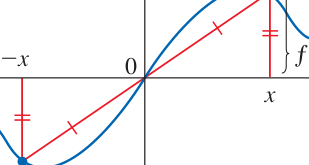
\includegraphics[width=\linewidth]{images/p0051_fig3.png}

    \vspace{0.33cm}
    \noindent{\color{stewartcyan}\rule{6pt}{6pt}}\hspace{6pt}\textbf{\large\textsf{Hàm số đồng biến và hàm số nghịch biến}}
    \vspace{0.16cm}

    \noindent Đồ thị trong Hình 22 đi lên từ $A$ đến $B$, đi xuống từ $B$ đến $C$, và đi lên trở lại từ $C$ đến $D$. Hàm số $f$ được gọi là \textbf{đồng biến} trên khoảng $[a, b]$, \textbf{nghịch biến} trên $[b, c]$, và đồng biến trở lại trên $[c, d]$. Lưu ý rằng nếu $x_1$ và $x_2$ là hai số bất kỳ nằm giữa...
\end{minipage}